

\fancypagestyle{miEstilo502}{
   \lhead{5.2 Descripción de los componentes y servicios}
   \rhead{Página \thepage}
   \lfoot{}
   \cfoot{}
   \rfoot{}
}

\pagestyle{miEstilo502}


\subsection{Descripción de los componentes y servicios} \label{sec:composer}

La aplicación (SIVIRA) desarrollada en este proyecto está compuesta por los siguientes componentes:

\subsubsection{Módulos}

Los módulos son un conjunto de funciones cuyo objetivo es encapsular funcionalidades que después serán utilizadas por el resto de componentes de la aplicación (ver figura \ref{img:modulos}). A continuación se realiza una descripción de cada uno de ellos.

\textbf{Logger}

Módulo cuyo objetivo es poder capturar y almacenar los logs de la aplicación en ficheros independientes para monitorizar el estado de la aplicación. Su implementación parte de una clase abstracta base, cuyo objetivo es definir las propiedades y métodos que tendrán todas las clases que implementarán los logs del sistema. 

\begin{figure}[h]
	\centering
	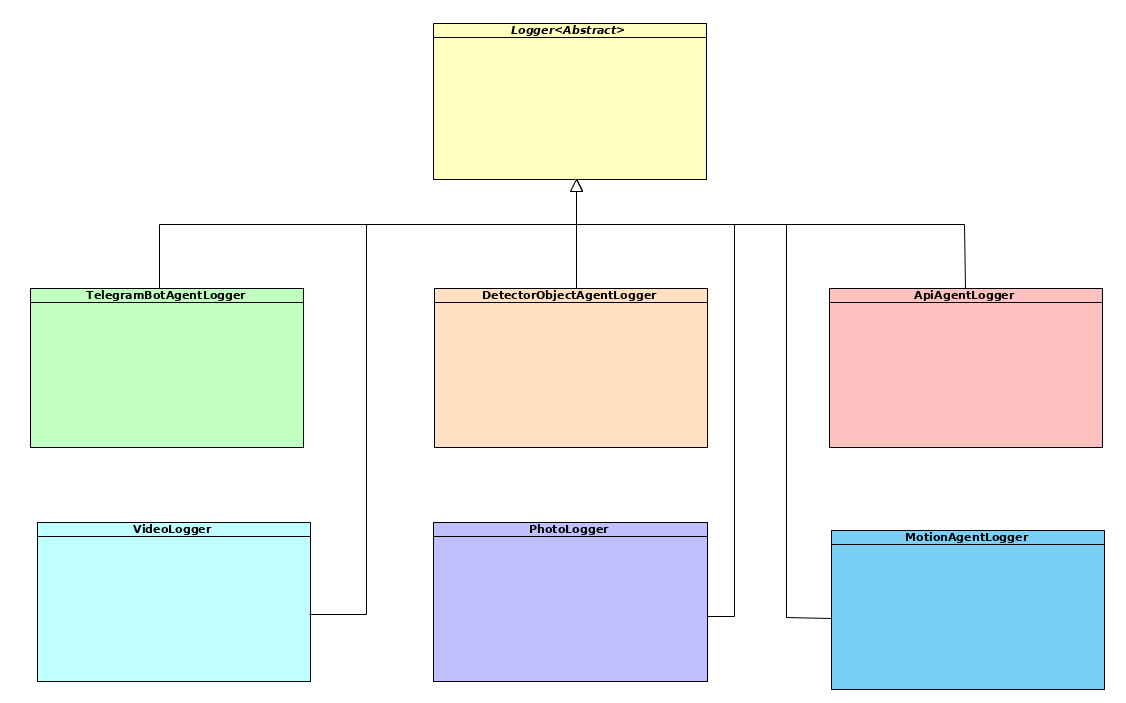
\includegraphics[scale=0.45]{images/83}
	\caption{Relación de herencia entre las clases logger}
\end{figure}

\newpage

Por defecto, los logs son mostrados y almacenados de la siguiente forma:

\begin{itemize}
\item \textbf{Consola}: Corresponde a la salida \texttt{stdout}. Todo los logs por encima de un nivel determinado de prioridad será mostrado por la salida de consola.

\item \textbf{Archivo de módulo}: Cada módulo y microservicio tendrán un fichero de log independiente para poder monitorizar su comportamiento a lo largo de su ejecución.

\item \textbf{Archivo de la aplicación}: La aplicación consta de un archivo de logs donde se almacenan todos los logs de módulos y microservicios de forma conjunta.

\item \textbf{Archivo de errores}: Todos los errores que surjan en cualquier módulo o microservicio son almacenados en este fichero para poder comprobar el estado de la aplicación.

\end{itemize}

Los niveles de logs que se han establecido son los siguientes:

\begin{itemize}

\item \textbf{DEBUG}: Nivel destinado a la depuración del código. Este nivel solo genera log en la salida por pantalla, y no se almacena en ningún fichero.

\item \textbf{INFO}: Nivel destinado a mostrar un mensaje informativo sobre alguna acción llevada a cabo. Estos logs son almacenados en el fichero de módulo correspondiente, en el fichero de logs de la aplicación y mostrados por pantalla.

\item \textbf{WARNING}: Nivel destinado a mostrar un mensajes de advertencia por posible mal uso de las llamadas a funciones, o simplemente porque algunas de ellas están '{deprecated}`. Estos logs son almacenados en el fichero de módulo correspondiente, en el fichero de logs de la aplicación y mostrados por pantalla.

\item \textbf{ERROR}: Nivel destinado a mostrar mensajes de error, que no son críticos para el sistema, y por lo tanto la aplicación sigue ejecutándose a pesar de producirse dichos errores. Estos logs son almacenados en el fichero de módulo correspondiente, en el fichero de logs de la aplicación, en el fichero de errores de la aplicación.

\item \textbf{CRITICAL}: Nivel destinado a mostrar mensajes de errores críticos que provocan el fallo de la aplicación. Estos logs son almacenados en el fichero de módulo correspondiente, en el fichero de logs de la aplicación, en el fichero de errores de la aplicación.

\end{itemize}



El formato por defecto de los logs es el siguiente:

\begin{itemize}
\item \textbf{Formato del archivo de errores}: \texttt{[Nivel:FechaHora:NombreArchivo:Función:Línea] Mensaje}. Por ejemplo:

\vspace{-1cm}

\begin{verbatim}

[ERROR:2019-08-15 13:10:11,597:logger.py:error:112x = set] Error while
trying to send an alert to Detector API agent with address 
http://192.168.1.100:11000.¿It is running?

\end{verbatim}


\vspace{-1cm}

\item \textbf{Formato del resto de logs}: \texttt{[Nivel:FechaHora] Mensaje}. Por ejemplo:

\vspace{-1.2cm}

\begin{verbatim}

[INFO:2019-08-13 18:35:03,278] A 5 seconds video is being 

\end{verbatim}

\end{itemize}

\vspace{-1.2cm}

Todos los ficheros de logs son almacenados en el directorio llamado \texttt{logs}. Dentro de dicho directorio, nos encontraremos los siguientes ficheros de logs:

\vspace{-0.4cm}

\begin{itemize}
\item \textbf{API\_agent.log}: Logs correspondientes a la API.
\item \textbf{detector\_object\_agent.log}: Logs correspondientes al agente detector de objetos.
\item \textbf{photo\_module.log}: Logs correspondientes al módulo de fotos.
\item \textbf{video\_module.log}: Logs correspondientes al módulo de vídeo.
\item \textbf{motion\_agent.log}: Logs correspondientes al agente detector de movimiento.
\item \textbf{security\_system\_PI\_app\_ERROR.log}: Logs correspondientes a los errores obtenidos por cualquier módulo o microservicio.
\item \textbf{security\_system\_PI\_app.log}: Logs correspondientes a los generados por módulos y microservicios a lo largo de su ejecución.
\item \textbf{telegram\_bot\_agent.log}: Logs correspondientes al bot de Telegram.

\end{itemize}

La implementación de este módulo puede comprobarse en este \href{https://github.com/jmv74211/TFM_security_system_PI/blob/master/src/modules/logger.py}{enlace}.

\textbf{Photo} 

Módulo que implementa la clase \texttt{Photo} con la que se pretende administrar el recurso de la cámara de la Raspberry PI para capturar fotografías, además de establecer los diferentes parámetros de la cámara como resolución, rotación \ldots

Esta clase añade una capa de abstracción a la biblioteca \texttt{PiCamera} \cite{ref12}, para permitir conectarse con el recurso de la cámara de forma personalizada.

Las funcionalidades que aporta este módulo son las siguientes:

\vspace{-0.5cm}

\begin{itemize}
\item Capturar una fotografía.
\item Realizar una captura secuencial de fotografías en un intervalo de tiempo
\item Establecer la configuración de la cámara: Rotación, resolución, giro horizontal o giro vertical.

\end{itemize}

\vspace{-0.5cm}

La implementación de este módulo puede comprobarse en este \href{https://github.com/jmv74211/TFM_security_system_PI/blob/master/src/modules/photo.py}{enlace}.

\textbf{Video} 

Módulo que implementa la clase \texttt{Video} con la que se pretende administrar el recurso de la cámara de la Raspberry PI para realizar grabaciones de vídeo, además de establecer los diferentes parámetros de la cámara como resolución, rotación \ldots

Esta clase añade una capa de abstracción a la biblioteca \texttt{PiCamera} \cite{ref12}, para permitir conectarse con el recurso de la cámara de vídeo de forma personalizada.

Las funcionalidades que aporta este módulo son las siguientes:

\vspace{-0.5cm}

\begin{itemize}
\item Realizar una grabación de vídeo.
\item Conversión de formato de vídeo \texttt{.h264} a \texttt{.mp4} (compatible con telegram).
\item Establecer la configuración: Rotación, resolución, giro horizontal, giro vertical y mostrar hora y fecha durante la grabación de vídeo. .

\end{itemize}

\vspace{-0.5cm}

La implementación de este módulo puede comprobarse en este \href{https://github.com/jmv74211/TFM_security_system_PI/blob/master/src/modules/video.py}{enlace}.

\textbf{Authentication} 

Módulo implementado para realizar una autenticación en el sistema. Esta autenticación es solicitada por la API, ya que junto a la petición deberán de ir las credenciales de acceso que se han definido en la configuración de la aplicación.

Este módulo básicamente implementa una función para poder comprobar si la autenticación es correcta. Su implementación puede comprobarse en este \href{https://github.com/jmv74211/TFM_security_system_PI/blob/master/src/modules/authentication.py}{enlace}.

\subsubsection{Servicios}

Los servicios son procesos destinados a realizar alguna tarea en concreto y enviar una petición o respuesta con los resultados a la API. A continuación se realiza una descripción de cada uno de ellos.

\textbf{Motion agent}

Este servicio se encarga de controlar el sensor de movimiento y detectar cuando es activado para poder manejar dicho evento y enviar una alerta a la API. Las tareas realizadas por este servicio son las siguientes:

\vspace{-0.5cm}

\begin{itemize}
\item Controlar el estado del sensor.
\item Capturar fotos o vídeos en caso de detectar algún tipo de movimiento.
\item Enviar una petición para procesar la imagen capturada, con el objetivo de poder detectar si hay alguna persona en ella.
\item Generar una alerta en la API en caso detectar a una persona en la foto.
\item Mover la foto generada por la alerta al directorio de \texttt{false\_positive} en caso de no detectar ninguna persona en la foto.

\end{itemize}

Para más información, en la sección \ref{sec:interac} se detallará como funciona e interacciona este servicio con el resto de elementos.

La implementación de este servicio puede comprobarse en este \href{https://github.com/jmv74211/TFM_security_system_PI/blob/master/src/agents/motion_agent.py}{enlace}.

\textbf{Object detector agent}

Este servicio se encarga de procesar una foto y devolver una lista de objetos detectados en dicha foto. Este servicio es usado por el \texttt{motion agent}, ya que cuando detecta movimiento (si la funcionalidad de detección de personas está activada), envía una petición a este servicio, y se le responde con la lista de objetos.

Esta funcionalidad ha sido implementada gracias al uso de la biblioteca de aprendizaje automático \texttt{Tensorflow} \cite{ref17}, ya que se ha utilizado para cargar el modelo preentrenado \texttt{ssdlite\_mobilenet\_v2\_coco} \cite{ref27} para poder predecir una lista de objetos que aparecen en una imagen.

El motivo por el cual se ha seleccionado ese modelo, es porque es el modelo más ligero, y el único viable para este proyecto en la Raspberry PI (debido a sus bajos recursos hardware). Antes de escoger este modelo, se hicieron pruebas con otros un poco más pesados y los resultados eran abrumadores. Utilizando otros modelos, se han obtenido una media de espera de más de 100 segundos para procesar la imagen (obviamente inviable).

Utilizar el modelo \texttt{ssdlite\_mobilenet\_v2\_coco} junto con una resolución de imagen media (1280x720) ha permitido obtener tiempos de procesamiento comprendidos entre unos 5 y 10 segundos, tiempo de espera que es aceptable.

El uso de este servicio es optativo, es decir, puede ser deshabilitado en las opciones o mediante la intefaz de usuario, y la aplicación puede funcionar normalmente. Es optativo por el hecho de que su uso implica una serie de ventajas e inconvenientes que puede hacer pensar si realmente vale la pena utilizar este servicio o no.

Personalmente, yo recomendaría usar este servicio, ya que hay casos en los que se quiere controlar una zona y puede que haya demasiados falsos positivos en las alertas por motivos como: animales domésticos, alta sensibilidad del sensor \ldots

A continuación se mencionan las posibles ventajas e inconvenientes de utilizar este servicio.

Ventajas

\begin{itemize}

\vspace{-0.5cm}

\item Evita posibles falsos positivos en las alertas generadas.
\item Puede aumentar el grado de eficacia del sistema de seguridad.
\end{itemize}

Desventajas

\vspace{-0.5cm}

\begin{itemize}
\item Añade sobrecarga de procesamiento en la Raspberry PI, calentamiento \ldots.
\item Añade latencia (5 a 10 segundos) en el momento de generar alertas, es decir, aumenta el tiempo desde que se produce un evento hasta que se envía la alerta.
\item Dado que el modelo de predicción es muy ligero, no es efectivo al 100\% y puede cometer algunos fallos.
\item Dificulta el proceso de instalación de la aplicación.
\end{itemize}

Por estos motivos, y porque la instalación de este agente puede resultar un poco tediosa (aunque todo está explicado en el repositorio del proyecto \cite{ref1}) se ha decidido proponer dos tipos de instalaciones, una en la que se utiliza otro servicio para filtrar eventos y reducir el número de falsos positivos en las alertas, y la otra en la que se prescinde totalmente de este servicio, y se genera una alerta tras la detección de cualquier movimiento.

La implementación de este servicio puede comprobarse en este \href{https://github.com/jmv74211/TFM_security_system_PI/blob/master/src/agents/object_detector_agent.py}{enlace}.

Para más información se puede consultar la \href{https://github.com/jmv74211/TFM_security_system_PI/blob/master/doc/api/object_detector_agent_doc.md}{documentación} sobre este servicio.

\textbf{Pistream}

\texttt{Pistream} es un servicio que se encarga de proporcionar un servidor de streaming y una interfaz web donde poder reproducirlo. Este servicio es activado y desactivado por la \texttt{API}, y consta de los siguientes componentes:

\begin{itemize}

\item \textbf{Servidor de streaming}: Componente para crear un servidor HTTP de streaming utilizando el protocolo \texttt{websocket} \cite{ref28}. Cuando es iniciado, levanta varias hebras para iniciar el protocolo \textbf{websocket}, el servidor HTTP y la retransmisión de vídeo. Está implementado en \texttt{Python}, y hace uso del componente \texttt{jsmpg.js} que implementa un conjunto de funciones de \texttt{Javascript}.

\item \textbf{jsmpg.js}: Conjunto de bibliotecas de \texttt{Javascript} utilizadas para realizar streaming sobre \texttt{websockets}.

\item \textbf{index.html}: Interfaz responsive implementada en \texttt{HTML},\texttt{CSS} para mostrar la retransmisión de vídeo a través del navegador. 

Es importante destacar que este servicio ha partido de la base de un proyecto open source \cite{ref29}, y que posteriormente se ha modificado y adaptado al ámbito de este proyecto.

\end{itemize}

Comentar que durante la fase de investigación de este servicio, estuve probando distintos proyectos similares cuyo objetivo era proporcionar las herramientas necesarias para proporcionar servicio de streaming de vídeo. Tras realizar varias pruebas, obtuve mejor rendimiento y calidad de servicio utilizando y adaptando el proyecto anteriormente mencionado \cite{ref29}.

En la sección \ref{sec:interac}, se mostrará como interacciona este servicio con el resto de componentes de la aplicación. Su implementación se puede comprobar en este \href{https://github.com/jmv74211/TFM_security_system_PI/tree/master/src/modules/pistream}{enlace}.

\subsubsection{API RESTful}

La \texttt{API} RESTful es el centro neurálgico de la aplicación. Una API RESTful \cite{ref30}, también conocida como servicio web RESTful, se basa en la tecnología de transferencia de estado de representación (REST) \cite{ref30}, un estilo arquitectónico y un enfoque de las comunicaciones que se utiliza a menudo en el desarrollo de servicios web.

La principal función de esta \texttt{API} es recibir peticiones HTTP haciendo uso de los verbos (GET,POST,PUT y DELETE), llevar a cabo una tarea, y finalmente devolver una respuesta. Esta \texttt{API} hace uso del conjunto de módulos (ver figura \ref{img:conexionapimodulos}) y se comunica directamente con el conjunto de servicios (ver figura \ref{img:conexionserviciosapi}) para llevar a cabo la tarea y enviar la respuesta al emisor (en este caso es el bot de telegram, pero podría ser cualquier otro proceso).

Esta \texttt{API} está implementada en Python3 utilizando la biblioteca de \texttt{flask} \cite{ref14}. Sus principales funcionalidades son las siguientes:

\begin{itemize}
\item Realizar una foto (asíncrono).
\item Realizar una grabación de vídeo (asíncrono).
\item Devolver el estado de una tarea creada de forma asíncrona.
\item Parar la ejecución de una tarea creada de forma asíncrona.
\item Activar, desactivar y comprobar el estado del servicio de detección de movimiento.
\item Comprobar y recibir alertas del servicio de detección de movimiento.
\item Activar, desactivar y comprobar el estado del servicio de streaming.
\item Leer la configuración de cámara realizada por el usuario: rotación, resolución \ldots
\end{itemize}

En la sección \ref{sec:interac}, se describirá como interacciona la \texttt{API} con el resto de componentes de la aplicación. La implementación de este servicio puede comprobarse en este \href{https://github.com/jmv74211/TFM_security_system_PI/blob/master/src/agents/api_agent.py}{enlace}.

Para más información se puede consultar la \href{https://github.com/jmv74211/TFM_security_system_PI/blob/master/doc/api/api_agent_doc.md}{documentación de la API}.

\subsubsection{Bot de telegram}

El \texttt{bot de telegram} es un proceso cuyo objetivo es recibir y enviar peticiones a la API de telegram \cite{ref31}, y hacer de intermediario entre el usuario y la \texttt{API} de la aplicación que se conecta con el conjunto de módulos y servicios de la aplicación (ver figura \ref{img:conexionbotapitelegram}).

Este bot de telegram ha sido implementado utilizando Python y una biblioteca llamada \texttt{pyTelegramBotAPI} \cite{ref13}. El conjunto de funcionalidades que aporta este bot son las siguientes:

\begin{itemize}
\item Activar o desactivar los siguientes modos: manual, automático o streaming.
\item Modificar la configuración de captura de fotos o grabaciones de vídeo: rotación,resolución, giro horizontal \ldots
\item Obtener ayuda sobre los comandos disponibles a usar.
\item Obtener credenciales de acceso de Telegram: nombre de usuario, id de usuario \ldots
\item Redireccionar a la documentación de la aplicación.
\item Activar, desactivar y comprobar el estado del agente detector de objetos.
\item Activar y desactivar el servidor de streaming.
\item Activar y desactivar el agente detector de movimiento.
\item Realizar capturas de fotografías.
\item Realizar grabaciones de vídeo especificando el número de segundos.
\end{itemize}

Todas estas funcionalidades son utilizadas por el usuario a través del bot. El principal medio de interacción por defecto es a través de comandos (por ejemplo \textit{/start}). Dado que el uso de comandos no puede ser lo más cómodo posible, e incluso puede ser díficil de recordar o utilizar, \textbf{se ha implementado una interfaz}, haciendo uso de los \texttt{botones callback} que permite usar la API de Telegram.

Simplemente, para que el usuario pueda interaccionar con la aplicación, solo es necesario que éste acceda en Telegram a la conversación del bot, escriba cualquier letra (o también el comando \textit{/start}) y automáticamente le aparecerá un menú de botones por el que podrá navegar y acceder al conjunto de funcionalidades de la aplicación.

Todas las funcionalidades y descripción de uso están descritas en el manual de usuario (de este documento), o también se puede consultar directamente en la documentación del repositorio de github \cite{ref1}.

También se puede consultar la implementación de este bot en este \href{https://github.com/jmv74211/TFM_security_system_PI/blob/master/src/agents/telegram_bot.py}{enlace}.
